\section{Data and MC samples}\label{sec:Zprime_data_mc}
The name and integrated luminosity of the all datasets used in this analysis are summarized in Table \ref{tab:Zprime-data-samples}. The DoubleEG dataset requires at least two trigger level electrons or photons for each event and it is used for main analysis. The SingleElectron dataset requires at least one trigger level electron for each event and it is used for trigger efficiency and electron selection efficiency measurement. The SingleMuon dataset requires at least one trigger level muon for each event and it is used for $\mathrm{t\bar{t}}$ background cross check using $\mathrm{'e\mu'}$ method. The SinglePhoton dataset requires at least one trigger level photon for each event and it is used for fake electron study. Form eras 2016B through 2016G and 2017B through 2017F the re-reconstruction datasets are used, the prompt reconstruction datasets are used for era 2016H. The total integrated luminosity of the data sample is 35.9$fb^{-1}$ and 41.4$fb^{-1}$ collected by the CMS experiment in 2016 and 2017 respectively. Only certified data which recommended for physics analysis is used.
\begin{table}[htp]
\small
\caption{Datasets (X) used in this analysis. X = DoubleEG is for the main analysis, X = SingleElectron is for trigger and electron selection efficiency, X = SinglePhoton is for the fake electron study and X = SingleMuon is for e$\mu$ study.\label{tab:Zprime-data-samples}}
\begin{center}
  \begin{tabular}{|c|l|c|}
    \hline
    Year& Datasets                               &   Integrated luminosity (\fbinv)       \\  \hline
        &/X/Run2016B-03Feb2017\_ver2-v2/MINIAOD  & $5.788$ \\
        &/X/Run2016C-03Feb2017-v1/MINIAOD        & $2.573$ \\
        &/X/Run2016D-03Feb2017-v1/MINIAOD        & $4.248$ \\
    2016&/X/Run2016E-03Feb2017-v1/MINIAOD        & $4.009$ \\
        &/X/Run2016F-03Feb2017-v1/MINIAOD        & $3.102$ \\
        &/X/Run2016G-03Feb2017-v1/MINIAOD        & $7.540$ \\
        &/X/Run2016H-03Feb2017\_ver2-v1/MINIAOD & $8.391$ \\
        &/X/Run2016H-03Feb2017\_ver3-v1/MINIAOD & $0.215$ \\ \hline
        &Sum 2016                               & $35.867$ \\ \hline

        &/X/Run2017B-17Nov2017-v1/MINIAOD  &  $4.802$ \\
        &/X/Run2017C-17Nov2017-v1/MINIAOD  &  $9.629$ \\
    2017&/X/Run2017D-17Nov2017-v1/MINIAOD  &  $4.235$ \\
        &/X/Run2017E-17Nov2017-v1/MINIAOD  &  $9.268$ \\
        &/X/Run2017F-17Nov2017-v1/MINIAOD  &  $13.433$ \\ \hline
        &Sum 2017                          &  $41.368$ \\ \hline

  \end{tabular}
\end{center}
\end{table}

The Monte Calor (MC) simulation samples used in the main analysis for 2016 and 2017 are summarized in Table \ref{tab:Z_mc-samples_1} with the corresponding cross section and the precision of the cross section. It is organized as follows for 2016 MC samples: the top part of the samples are for Drell-Yan (DY) process simulation which is the main background in this analysis, then it is followed by $t\bar{t}$ process simulation samples and then is for di-boson (WW, WZ, ZZ) process simulation samples, finally is for gravitation signal simulation sample. Similar organization for 2017 MC samples. The 2016 MC samples are produced from RunIISummer16MiniAODv2*PUMoriond17\_80X\_mcRun2\_asymptotic\_2016\_TrancheIV\_v6 campaign and for 2017 it is from RunIIFall17MiniAOD-94X\_mc2017\_realistic\_v10\_v1(v2) campaign.
The most samples are generated by POWHEG v2 ~\cite{Nason:2004rx,Frixione:2007vw,Alioli:2010xd,Alioli:2008gx,Frixione:2007nw,Re:2010bp} at next-to-leading order (NLO), few are generated by MadGraph5\_aMC@NLO~\cite{MadGraph5} at NLO. The Pythia8 ~\cite{Sjostrand:2014zea} is used to simulate the parton showering and hadronization. For detector response it is simulated by Geant4 ~\cite{Agostinelli:2002hh}.


\begin{table}[htp]
  \begin{center}
\small
\smallskip\noindent
\resizebox{\linewidth}{!}{%
\begin{tabular}{|c|l|l|l|l|}
\hline
Year & Sample                                                         & xsection(pb) & xs precision  \\ \hline
\multirow{29}{*}{2016} &ZToEE\_NNPDF30\_13TeV-powheg\_M\_50\_120                 & 1975         & NLO                \\
&ZToEE\_NNPDF30\_13TeV-powheg\_M\_120\_200                & 19.32        & NLO                  \\
&ZToEE\_NNPDF30\_13TeV-powheg\_M\_200\_400                & 2.73         & NLO                 \\
&ZToEE\_NNPDF30\_13TeV-powheg\_M\_400\_800                & 0.241        & NLO                 \\
&ZToEE\_NNPDF30\_13TeV-powheg\_M\_800\_1400               & 1.68E-2      & NLO                 \\
&ZToEE\_NNPDF30\_13TeV-powheg\_M\_14000\_2300             & 1.39E-3      & NLO                \\
&ZToEE\_NNPDF30\_13TeV-powheg\_M\_2300\_3500              & 8.948E-5      & NLO                 \\
&ZToEE\_NNPDF30\_13TeV-powheg\_M\_3500\_4500              & 4.135E-6      & NLO                 \\
&ZToEE\_NNPDF30\_13TeV-powheg\_M\_4500\_6000              & 4.56E-7      & NLO                \\
&ZToEE\_NNPDF30\_13TeV-powheg\_M\_6000\_Inf               & 2.06E-8      & NLO                 \\
&DYJetsToLL\_M-50\_TuneCUETP8M1\_13TeV-amcatnloFXFX-pythia8 (for Z $\rightarrow$ $\tau\tau$) & 5765.4       & NNLO             \\\cline{2-4}
&TTTo2L2Nu\_TuneCUETP8M2\_ttHtranche3\_13TeV-powheg        & 87.31        & NNLO                      \\
&TTToLL\_MLL\_500To800\_TuneCUETP8M1\_13TeV-powheg-pythia8  &   0.326            &NLO            \\
&TTToLL\_MLL\_800To1200\_TuneCUETP8M1\_13TeV-powheg-pythia8  &  3.26E-2             &NLO           \\
&TTToLL\_MLL\_1200To1800\_TuneCUETP8M1\_13TeV-powheg-pythia8  & 3.05E-3              &NLO          \\
&TTToLL\_MLL\_1800ToInf\_TuneCUETP8M1\_13TeV-powheg-pythia8  &  1.74E-4             &NLO           \\
&ST\_tW\_top\_5f\_NoFullyHadronicDecays\_13TeV-powheg\_TuneCUETP8M1/         & 19.47         & app.NNLO           \\
&ST\_tW\_antitop\_5f\_NoFullyHadronicDecays\_13TeV-powheg\_TuneCUETP8M1/     & 19.47         & app.NNLO           \\\cline{2-4}
&WWTo2L2Nu\_13TeV-powheg                                        & 12.178       & NNLO                    \\
&WWTo2L2Nu\_Mll\_200To600\_13TeV-powheg                         & 1.39     & NNLO                 \\
&WWTo2L2Nu\_Mll\_600To1200\_13TeV-powheg                        & 5.7E-2    & NNLO                    \\
&WWTo2L2Nu\_Mll\_1200To2500\_13TeV-powheg                       & 3.6E-3    & NNLO                    \\
&WWTo2L2Nu\_Mll\_2500ToInf\_13TeV-powheg                        & 5.4E-5      & NNLO                  \\
&WZTo3LNu\_TuneCUETP8M1\_13TeV-powheg-pythia8 &    4.42965 & NLO                \\
&WZTo2L2Q\_13TeV\_amcatnloFXFX\_madspin\_pythia8 &    5.595& NLO                \\
&ZZTo2L2Nu\_13TeV\_powheg\_pythia8 &   0.564& NLO                \\
&ZZTo4L\_13TeV\_powheg\_pythia8 &     1.212 & NLO                \\
&ZZTo2L2Q\_13TeV\_powheg\_pythia8 &    1.999& NLO                \\\cline{2-4}
&RSGravToEEMuMu\_kMpl-001\_M-*\_TuneCUEP8M1\_13TeV-pythia8               & -            & -                               \\\hline
\multirow{17}{*}{2017}&ZToEE\_NNPDF31\_13TeV-powheg\_M\_50\_120                & 1975         & NLO                \\
&ZToEE\_NNPDF31\_13TeV-powheg\_M\_120\_200                & 19.32        & NLO                  \\
&ZToEE\_NNPDF31\_13TeV-powheg\_M\_200\_400                & 2.73         & NLO                 \\
&ZToEE\_NNPDF31\_13TeV-powheg\_M\_400\_800                & 0.241        & NLO                 \\
&ZToEE\_NNPDF31\_13TeV-powheg\_M\_800\_1400               & 1.68E-2      & NLO                 \\
&ZToEE\_NNPDF31\_13TeV-powheg\_M\_14000\_2300             & 1.39E-3      & NLO                \\
&ZToEE\_NNPDF31\_13TeV-powheg\_M\_2300\_3500              & 8.948E-5      & NLO                 \\
&ZToEE\_NNPDF31\_13TeV-powheg\_M\_3500\_4500              & 4.135E-6      & NLO                 \\
&ZToEE\_NNPDF31\_13TeV-powheg\_M\_4500\_6000             & 4.56E-7      & NLO                \\
&ZToEE\_NNPDF31\_13TeV-powheg\_M\_6000\_Inf              & 2.06E-8      & NLO                 \\
&DYJetsToLL\_M-50\_TuneCP5\_13TeV-amcatnloFXFX-pythia8 (for Z $\rightarrow$ $\tau\tau$) & 5765.4       & NNLO             \\\cline{2-4}
&TTTo2L2Nu\_TuneCP5\_PSweights\_13TeV-powheg-pythia8        & 87.31        & NNLO                      \\
&ST\_tW\_top\_5f\_NoFullyHadronicDecays\_TuneCP5\_13TeV-powheg-pythia8         & 19.47         & app.NNLO           \\
&ST\_tW\_antitop\_5f\_NoFullyHadronicDecays\_TuneCP5\_13TeV-powheg-pythia8     & 19.47         & app.NNLO           \\\cline{2-4}
&WW\_TuneCP5\_13TeV-pythia8                                         & 118.7        & NLO                      \\
&WZ\_TuneCP5\_13TeV-pythia8                                         & 47.13        & NLO                      \\
&ZZ\_TuneCP5\_13TeV-pythia8                                         & 16.523       & NLO                      \\\hline
\end{tabular}}
\caption{MC samples used in main analysis}
\label{tab:Z_mc-samples_1}
  \end{center}
\end{table}



The pile up distributions for MC and data which is calculated by using 69.2 mb as the minimum bias cross section are shown in Figure \ref{fig:Z_pileup} for 2016 and 2017. The average number of pile up in 2016 (2017) is 27 (33). MC events are re-weighted to account for the pile up difference between data and MC.
\begin{figure}[h!]
  \centering
	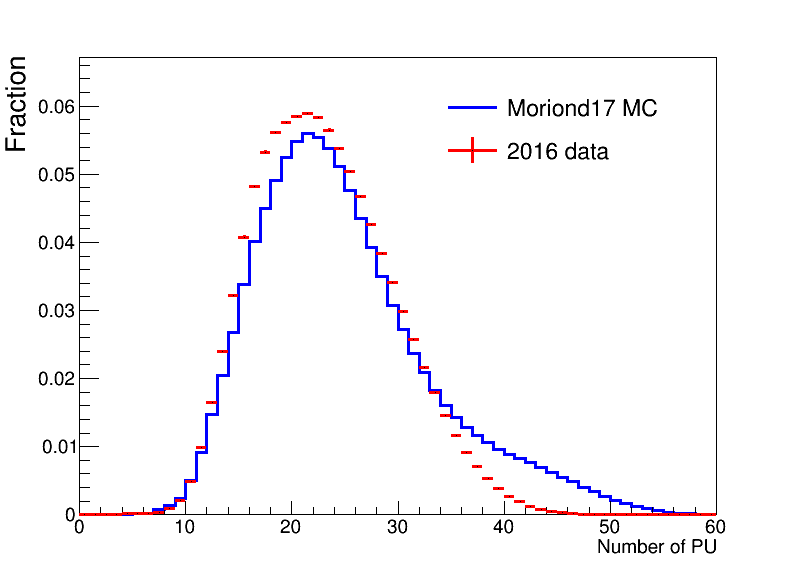
\includegraphics[width=0.45\textwidth]{figures/Zprime/PU.png}
    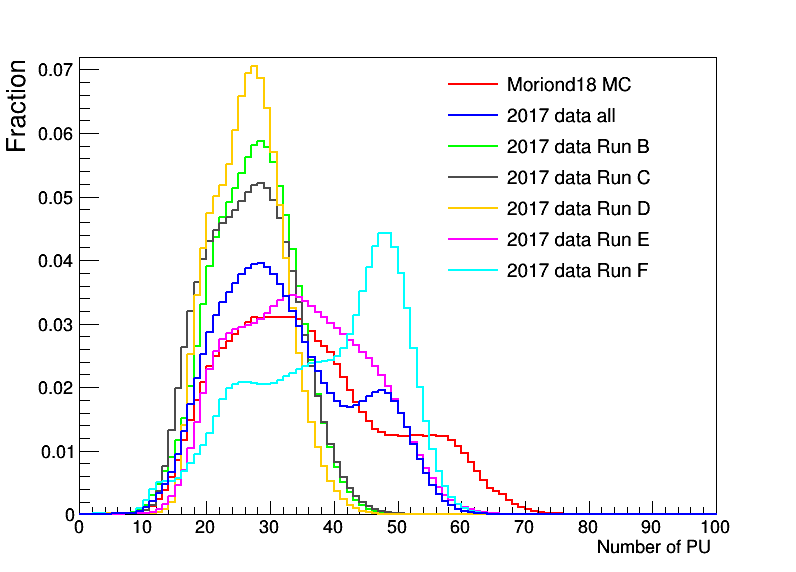
\includegraphics[width=0.45\textwidth]{figures/Zprime/2017_PU.png}
\caption{Pileup distribution for data and MC samples in 2016 (left) and in 2017 (right) .
 \label{fig:Z_pileup}}
\end{figure}

In order to improve data-mc agreement, in 2016 the data energy scale has been corrected by 1.0012 in the barrel and 1.0089 in the endcap using the mean values of the official EGamma scale corrections (except in Section \ref{sec:mass_res} study which we measured the mean data energy correction and found it agree with offical EGamma value). In 2017 the official EGamma energy scale in data and energy smearing in MC is applied in all studies.


